% gjilguid2e.tex
% V2.0 released 1998 December 18
% V2.1 released 2003 October 7 -- Gregor Hutton, updated the web address for the style files.

\documentclass{gji}
\usepackage{timet}
\usepackage{amsmath}
\usepackage{graphicx}


\graphicspath{{./paper_figures/placeholders/}}



\title[Comparisons of surface wave amplitude decays]
  {Comparisons of surface wave amplitude decays \\for colocated rotation and translation measurements}
\author[Bryant Chow]
  {Bryant Chow$^1$\thanks{Now at Victoria University of Wellington, Wellington, New Zealand}, 
  Heiner Igel$^1$, 
  Joachim Wassermann$^1$,
  Bernhard Schuberth$^1$,
  Celine Hadziiannou$^2$,
  Stefanie Donner$^3$,\\
  $^1$ Department of Earth and Environmental Sciences, Ludwig-Maximilians-University Munich, Theresienstra\ss e 41, D-80333 Munich, Germany.\\
  $^2$ Department of Earth Science, University of Hamburg, Hamburg, Germany\\
  $^3$ Federal Institute for Geosciences and Natural Resources, Hannover, Germany \\E-mail: bryant.chow@vuw.ac.nz
  }
\date{}
\pagerange{\pageref{firstpage}--\pageref{lastpage}}
\volume{}
\pubyear{}

%\def\LaTeX{L\kern-.36em\raise.3ex\hbox{{\small A}}\kern-.15em
%    T\kern-.1667em\lower.7ex\hbox{E}\kern-.125emX}
%\def\LATeX{L\kern-.36em\raise.3ex\hbox{{\Large A}}\kern-.15em
%    T\kern-.1667em\lower.7ex\hbox{E}\kern-.125emX}
% Authors with AMS fonts and mssymb.tex can comment out the following
% line to get the correct symbol for Geophysical Journal International.
\let\leqslant=\leq

\newtheorem{theorem}{Theorem}[section]

\begin{document}

\label{firstpage}

\maketitle

\begin{summary}
Current broad-band surface wave magnitude equations relate magnitude with station-receiver distance and the vertical component of peak ground velocity, such that only contributions from the vertical component of Rayleigh waves are present. With the advent of rotational ground motion data from instruments such as ring laser gyroscopes and fiber-optic gyroscopes, it is possible to determine peak amplitudes of rotations about the vertical axis, which is theoretically only sensitive to the transverse nature of Love waves, unaffected by the horizontal component of Rayleigh waves. We use this concept to study the amplitude decay of rotations versus translations, and determine the necessity of a separate surface wave magnitude equation for Love waves. Utilizing a large database of rotation ground motion events, collected in Wettzell, Germany, we empirically define decay constants for measured observables: rotation rate, rotation, vertical velocity and transverse velocity. Results indicate that measured rotation amplitudes decay faster over distance compared to velocity amplitudes, both on vertical and transverse components. Observations are corroborated with synthetic seismograms produced on a full scale 3D global model with crustal and Moho topography models. Synthetics were created with the spectral-element method Salvus, and suggest that ...
\end{summary}

\begin{keywords}
magnitude, rotational ground motions, seismic instrumentation, amplitude decay
\end{keywords}

\section{Introduction} 
% rotations are gaining traction, large catalog of events
For over a decade, the application of ring laser gyroscope technology to the field of seismology has allowed for near-continuous, direct, measurements of rotational ground motions. An ever growing number of observations from seismic events of varying size, distance and source mechanism, has been collected in an expansive catalog of waveform recordings for both direct rotation, and collocated translation measurements.
%> we routinely compare amplitude ratios for phase velocities
Previous work on this unique waveform dataset includes phase comparisons of translations and rotations with estimations of horizontal phase velocities [Igel 2005] %cite
automatic standardized processing of rotation and translation data [Salvermoser 2017],
variations of surface wave energy in oceanic microseisms [Tanimoto ????],. [More citations here?] %cite
Much of this preceding work however, focuses on single events, or collections of non-earthquake sources. This paper, on the other hand, aims to utilize a large portion of the dataset.

%> we want to understand how rotations decay compared to translations
%> how do we do this? we make 'magnitude scales' to quantify decay characterstics
%> these are not real magnitudes because we are geographically biased and we are not avera
%ging over hundreds of instruments like is common
In this paper, we aim to characterize and understand the differences in amplitude decay behavior of rotational and translational ground motion for a large number of seismic events. To do this, we make use of a sizable catalog of earthquake data, as measured by an observatory based ring laser gyroscope, and collocated broadband translation sensor. By processing rotation and translation observations in a near identical manner, we hope to directly compare results over a large set of event magnitudes, epicentral distances and  azimuths. We additionally seek to use this information to better understand decay characteristics of Love and Rayleigh waves.

This paper builds on work previously addressed by Igel et al. 2007, %cite igel 2007
where the question was posed: whether observed peak rotation amplitudes matched with expected values given by the surface wave magnitude equation. At the time, a limited number of recorded events lead to a small sample size. With a much larger number of events now currently available, we attempt to readdress this question, while also approaching the problem from the unique perspective of deriving magnitude scales to quantify and compare the decay characteristics of rotations and translations. Due to the uniqueness of our instrumental setup, we are restricted to observations at a single point of measurement. In order to provide comparisons to our observations, global 3D synthetic simulations were run with the wave propagation code Specfem3D Globe. Real seismic event locations, source parameters, and station locations are used, in order to provide the most comparable synthetic setup to observations. 

With these observations, we aim to make quantitative statements on surface wave amplitude decay, as well as to provide magnitude scale equations that may prove useful in determining expected rotation amplitudes from seismic events.

\subsection{Rotational Ground Motions}
Rotational ground motions induced by seismic events can currently be observed through direct measurement, and through array analysis of translation sensors [Spudich ????].
In the latter, spatial gradients are taken for measurements in an adequately spaced array of translation sensors, in order to derive components of the strain tensor [Spudich ?]. A downfall of array based methods, however, is the necessity for multiple instruments with known calibrations, and the importance of array spacing and geometry in the clarity of the recorded signal. With unique instrument designs, however, direct gradient measurements are also possible [Schreiber? Others?]. %different rotation sensors

Data for this study was recorded by the Gro\ss ring (G-ring) [Schreiber 2005, 2006], a 4x4m helium-neon ring laser gyroscope, located in Wettzell, Germany (49.144$^\circ$N, 12.87$^\circ$E). The G-ring operates on the principle of Sagnac interferometry [Stedman, 1997], which relates interference of counter propagating light beams to absolute rotation rate, through the following equation, 

\begin{equation}\label{eq:sagnac}
	\delta f = \frac{4A}{\lambda P}\mathbf{n}\cdot \mathbf{\Omega},
\end{equation}

\noindent where the constants are given by instrument area A, perimeter P and operating light wavelength $\lambda$. Equation \ref{eq:sagnac} relates an observable beat frequency $\delta f$ [Hz] to absolute rotation rate [rad/s] $\Omega$.

It is important to note that given stable instrument geometry and lasing, changes to the beat frequency $\delta f$, can only be introduced by changes to the inner product of the plane normal {\bfseries n} with the rotation rate direction $\mathbf{\hat{\Omega}}$ (e.g. through instrumental tilt), and through externally induced rotations (e.g. the passing of seismic waves). It has been shown that changes to the inner product as produced by tilt are one to two orders of magnitude smaller than rotations produced by passing seismic waves [Igel ????] [Schreiber ????], this provides unique benefit that G is theoretically insensitive to translations, and only sensitive to externally induced rotations.

\subsubsection{Phase velocity relation}\label{phasevel}
As shown in previous theoretical considerations towards measured rotations [Igel 2005], %citation
for a simple plane wave, the amplitudes of vertical rotation rate $\Omega_z$  and transverse acceleration $\ddot{u}_t$ can be related through the equation 

\begin{equation}\label{phasevelocity}
	\frac{\ddot{u}_t}{\Omega_z} = -2c,
\end{equation}

\noindent where c represents an apparent horizontal phase velocity. This relationship shows that, given a sufficient event-receiver distance (allowing a plane wave assumption), measured rotations are sensitive to the transverse component of translation, represented in teleseismic waves by surface horizontal waves (i.e. SH or Love waves). It also shows that waveforms of transverse acceleration and vertical rotation rate should theoretically be in phase, with oppositely polarized amplitudes, for passing horizontal waves. This can be seen in Figure \ref{fig:rr_ta}, showing two superimposed traces of rotation rate and transverse acceleration (filtered at T=20 s) for G and a colocated broad band seismometer. Following Equation \ref{phasevelocity}, a value of 3.81 km/s is calculated, which matches well with previous findings of phase velocity for this area [Igel 2007].

%In this paper the shortest epicentral distances considered are 2$^\circ$. A surface wave moving at a velocity of 4 km/s, with dominant period $T=20$s, covers 80 km per wavelength. As a rule of thumb, if 1$^\circ$ epicentral distance covers ~100 km distance, this gives two wavelengths as the shortest propagation distance. 


\begin{figure}
\centerline{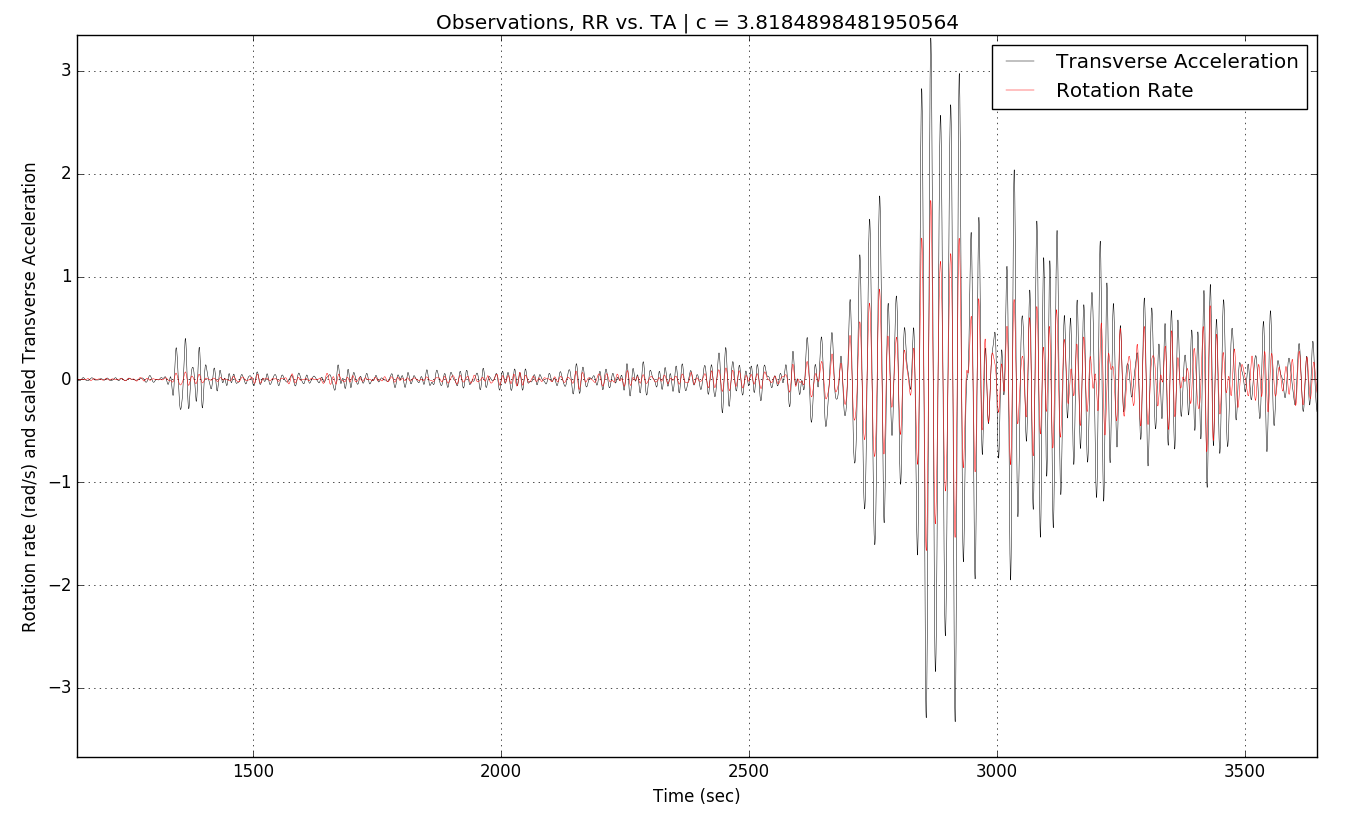
\includegraphics[width=0.5\textwidth]{rr_ta}}
\caption{Teleseismic event filtered at dominant period 20s. Note the phase matching of transverse acceleration and rotation rate, as well as the calculated value of horizontal phase velocity, c=3.81 km/s.}
\label{fig:rr_ta}
\end{figure}

\subsubsection{Peak correlation coefficient}
Correlations are a useful measure of similarity between two signals. It has been shown previously that for collocated measurements of vertical rotation rate and transverse acceleration, high values ($>0.9$) of zero lag correlations can be obtained in time windows centered around surface wave arrivals. %citation
Zero lag correlation coefficients are routinely computed for events measured by G [Salvermoser 2017], %citation
and are used in this study as a filtering tool to highlight "bad" events that exhibit low signal to noise ratios, or dissimilar waveforms which may arise due to non-physical effects (e.g. instrumental effects). Here, the largest correlation coefficient obtained for a seismogram is labeled the peak correlation coefficient (PCC), and is used as a representation of data quality for an event.


\subsection{Magnitude scales}
Here we discuss the common magnitude scale equation, and propose using a modified version of the equation as a method for comparing amplitude decay of various observables. Amplitude based magnitude scales provide empirically derived relationships between maximum trace amplitudes and source-receiver distances. Magnitude scales offer useful and quick estimates of relative sizes of earthquakes in a simple, standard  manner. 
The International Association of Planets Seismology and Earths Interior (IASPEI) Working Group on Magnitudes  proposed a modified version of the original surface wave magnitude equation proposed by Karnik et al. and Vanek et al., %citation
which is compatible for use with modern day broadband seismic instruments [Borrmann \& Bergman 2000].

In this work, we adhere strictly to these standard procedures provided by IASPEI as an outline for defining our own empirical magnitude scales. In turn, we use these derived scales as a tool for quantifying amplitude decay for different measured observables.

\subsubsection{Standard Procedures}\label{standproc}
The Working Group on Magnitudes' standard procedures gives the revised surface wave magnitude equation for broad-band instruments as,
\begin{equation}\label{eq:mag}
	M_S^{BB} = log_{10}(V/2\pi) + B\cdot log_{10}(\Delta) + C, 
\end{equation}
where the constants $B=1.66$ and $C=0.3$ control amplitude decay and order of magnitude, respectively. The parameter V should be the maximum trace amplitude (in nanometers second$^{-1}$) in the surface wave train, for a seismogram proportional to velocity, measured on the vertical component. 

Further criteria given by IASPEI posit that the period of the surface wave should lie within 3 s $\le$ T $\le$ 60 s, while epicentral distances should be between 2$^\circ \le \Delta \le 160^\circ$. It is further recommended that only shallow focus earthquakes should be considered, as medium to deep events are less capable of generating strong surface waves. %citation
Maximum trace amplitudes are described as one half the largest peak to adjacent trough deflection, and associated period are given as two times the temporal difference between peak and adjacent trough. All events and processing steps in this paper adhere to these guidelines.

\subsubsection{Instrumental proxies for Love and Rayleigh waves}\label{proxy}
A standard procedure for determining surface wave magnitude scales is to take amplitudes measured on the vertical component of translation. This is because vertical translation should only be sensitive to the vertical motions of Rayleigh waves, whereas vector sums of horizontal components can be influenced by both Love and Rayleigh waves. In the same vein, velocity measured on the transverse component should only show sensitivity to Love waves (and radial components should only be sensitive to the horizontal component of Rayleigh waves). This is, however not common practice,  due to the necessity of rotating horizontal components to the correct azimuth, which can be affected by ray paths and local site effects. The G-ring, which is: 1) insensitive to translations and 2) proportional in phase and amplitude to transverse acceleration, should however only be sensitive to Love waves in the surface wave train, irrespective of azimuth.  

In this study we use our instruments as physical wave-filters, in order to separate phases in the surface wave train. This allows us to study the influences of Love waves and Rayleigh waves individually. By comparing the vertical and transverse components of translations, to the vertical component of rotation, we can understand, by proxy, the wave types they are sensitive to.

\subsubsection{Application of rotations to magnitude scales}
The surface wave magnitude equation is defined for peak vertical velocity amplitudes in the surface wave train. In order to give a fair comparison using derived magnitude scales, a complementary rotation parameter is necessary. In Section \ref{phasevel}, an equation is given that relates rotation rates $\Omega$ with accelerations $\ddot{u}$. It would make the most sense, then, to compare velocities $\dot{u}$ with rotations $\omega$ (by integrating both sides). However, without previous work to draw precedence from, and for completeness, we present observations of both rotations and rotation rates in this study.

\section{Event choice}
The G-ring has been continuously recording at its current resolution since May, 2009 [Citation for mirror upgrade?]. 
The time range for events used in this study spans June 1, 2009 to September 1, 2016. An initial earthquake catalog was fetched from the Harvard Global Centroid Moment Tensor (GCMT) [Ekstr\"om et al. 2012 ?], %citation 
with events filtered by acceptable magnitude, source depth and epicentral distance from Wettzell, Germany. At this point we imposed the restriction that the derived 'magnitude' as given by our magnitude equations, should fall as close to the given surface wave magnitude as possible. This ensures that our derived scales do not stray too far from established scales. This meant that only events with centroid moment magnitude values of $6 \le M_{\text{wc}} < 8$ (as published in the GCMT catalog), were considered;   surface wave magnitude and moment magnitude are approximately equal in this range [Shearer 2009]. %citat
Zero-lag cross correlations of transverse acceleration and rotation rate were taken in order to calculate peak correlation coefficients (Section \ref{sec:dataproc}). Events were not considered if their peak correlation coefficient did not meet the criterion PCC $< 0.7$. 

These choices for event criteria narrowed the catalog down to roughyl 500 events in the given time period. Each event was appropriately filtered and processed (Section \ref{sec:dataproc}), and waveforms were individually inspected. Waveforms that exhibited anomalous behavior (i.e. unexpected high amplitude peaks outside the surface wave train, high signal-to-noise ratio etc.) were rejected. A final event catalog of 243 events was reached, shown on a world map in Figure \ref{fig:event_map}.

\begin{figure*}
\centerline{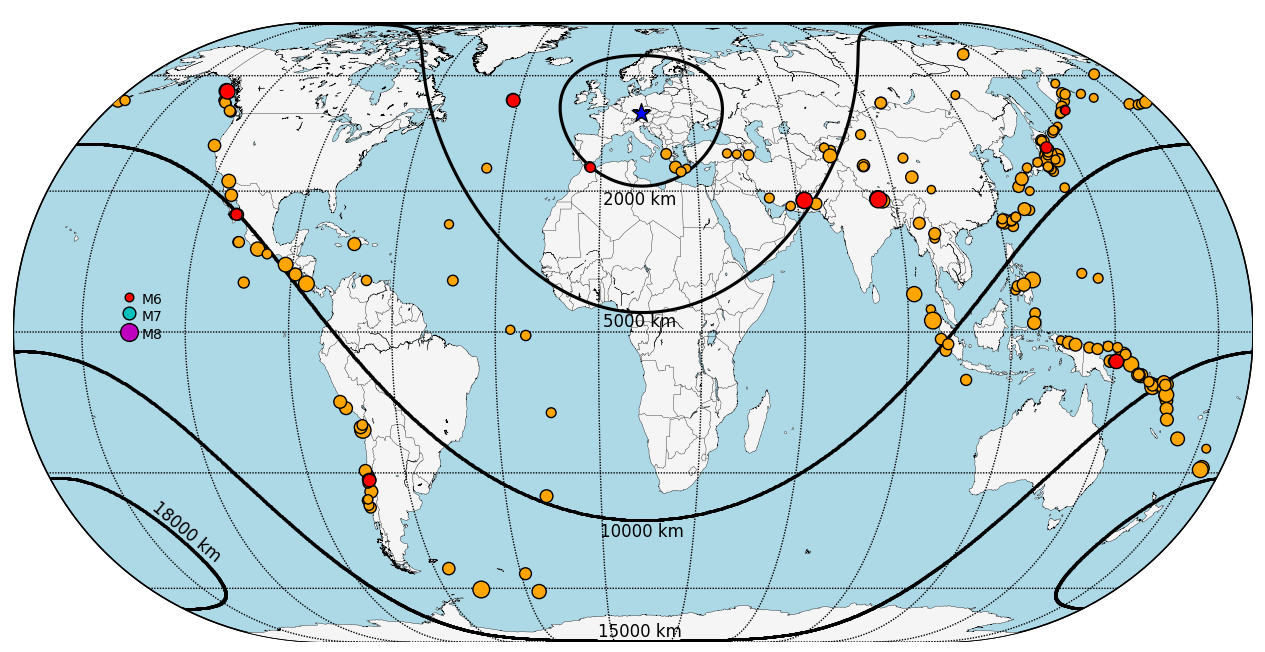
\includegraphics[width=.8\textwidth]{event_map}}
\caption{Event map. Size represents moment magnitude (M$_{wc}$). Orange dots show observed earthquakes used in magnitude scale derivation. Red dots show the ten events chosen for generation of synthetic seismograms. Black lines are equidistant points from the blue star, which represents the location of G in Wettzell, Germany (49.144$^\circ$N,12.87$^\circ$E).}
\label{fig:event_map}
\end{figure*}

\section{Methods}
\subsection{Data Processing}\label{sec:dataproc}
Events were processed in a similar fashion as the processing outlined in Salvermoser 2017. %cite johannes
Raw, continuous translation data in North, East and vertical components, as well as vertical rotation rate data, was fetched based on event origin time. Instrument response correction produced translation seismograms proportional to units of velocity (nm s$^{-1}$). Epicentral distances ($\Delta$) and theoretical backazimuth values were calculated from station-receiver latitude longitude pairs, and events were separated into categories of close ($\Delta < 3^\circ$), local ($\Delta <100^\circ$) and far ($\Delta \ge 100^\circ$). Horizontal components were rotated into the transverse, radial, vertical coordinate system by the appropriate theoretical backazimuth. Measurements from ring laser gyroscope instruments do not require frequency dependent instrument correction [Sagnac ????], %citation
therefore only a simple scale factor was necessary to retrieve seismograms proportional to rotation rate (nrad s$^{-1}$). Rotation rate traces were integrated to provide measurements of rotation (nrad), and transverse velocity was integrated to retrieve transverse acceleration, which was subsequently used to calculate correlations with vertical rotation rates.
A bandpass filter was applied to all traces for periods between 3 s $\le$ T $\le$ 60 s, in accordance to the IASPEI standard procedures. Peak amplitudes were chosen by finding minimum and maximum trace values and the largest associated peak or trough, respectively. The larger of the two was chosen, alongside the associated arrival time and dominant period, taken as two times the distance between peak and adjacent trough. 
Theoretical considerations used to restrict search to the surface wave train proved inconsistent over a large number of events, so maximum amplitudes in the entire trace were considered. Through manual inspection, picked amplitudes that fell outside the surface wave train (which occurred very infrequently) were rejected. An example of the waveforms and amplitude picking is shown in Figure \ref{fig:obswave}.


\begin{figure}
\centerline{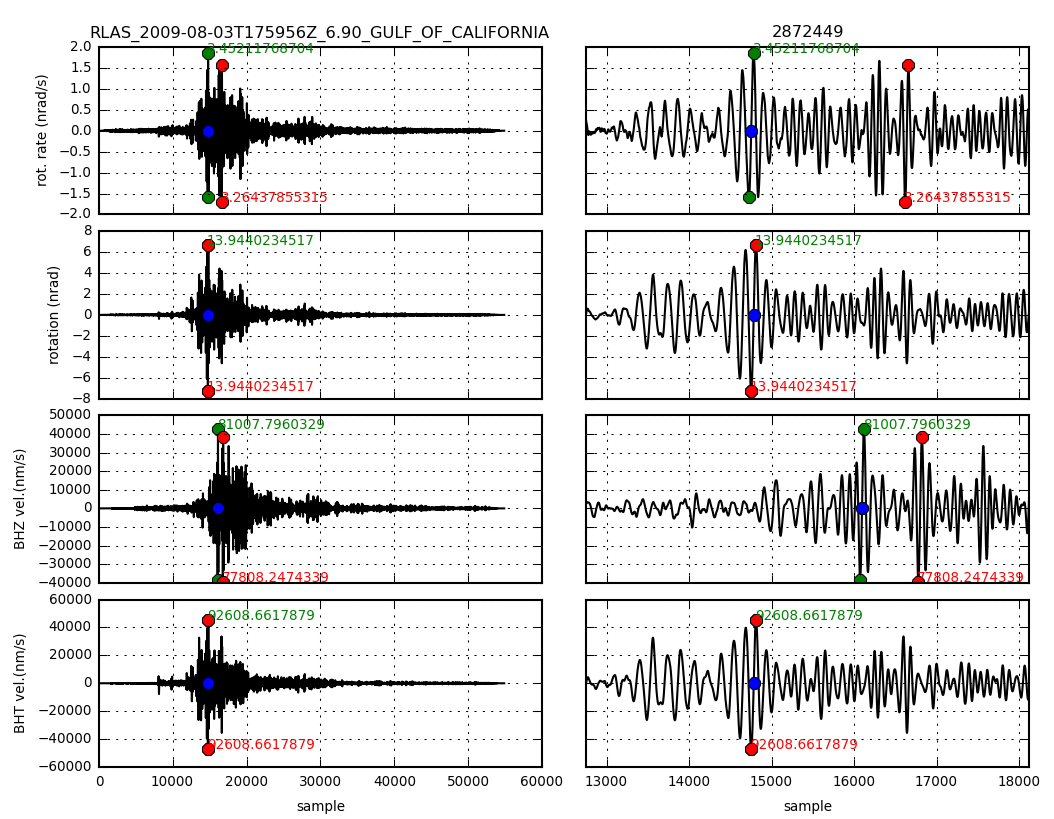
\includegraphics[width=0.5\textwidth]{observation_waveforms}}
\caption{Left: Seismograms for observed rotation rate, rotation (measured by G), and two components of translation (colocated STS-2), vertical and transverse components.\newline Right: Zoomed in section of seismograms, showing peak to peak amplitude choice (blue dot). Red and green dots show largest peak to adjacent trough distance and largest trough to adjacent peak distance, respectively. Note the visible difference in arrival times of the Love wave (as seen on rotation and transverse components), and the later arriving Rayleigh wave (as seen on the vertical component). }
\label{fig:obswav}
\end{figure}


\subsubsection{Zero-lag correlations}
To calculate peak correlations, traces of transverse acceleration and vertical rotation rate were segmented into small time windows based on the event-station distance. In each time window, a zero-lag correlation was performed, and a single value of correlation produced. From the entire trace, the max value was taken to represent the peak correlation coefficient. For most waveforms, the peak correlation coefficient lie in the surface wave train. As mentioned previously, these peak correlation values are used extensively as a ranking system for events, providing a quickly attainable measure of waveform quality.

\subsection{Curve fitting}
To quantify amplitude decay, magnitude scale coefficients were fit to the data using a simple linear regression. Equation \ref{eq:mag} represents a relationship between magnitude and amplitude for a single event. Using Equation \ref{eq:mag}, a collection of $n$ events can be represented in the form, 
\begin{equation}
	\begin{pmatrix}
		log_{10}(\Delta_{1}) & 1 \\
		log_{10}(\Delta_{2}) & 1 \\
		\vdots  & \vdots \\
		log_{10}(\Delta_{n}) & 1 
	\end{pmatrix}
	\begin{pmatrix}
		{B}\\
		{C}
	\end{pmatrix}
	=
	\begin{pmatrix}
		M_{\text{wc}_1} - log_{10}({V_1}/{2\pi})_{\text{max}} \\
		M_{\text{wc}_2} - log_{10}({V_2}/{2\pi})_{\text{max}} \\
		\vdots  \\
		M_{\text{wc}_n} - log_{10}({V_n}/{2\pi})_{\text{max}}
	\end{pmatrix},
	\label{eq:linearreg}
\end{equation}

\noindent which can be further condensed to the form, $\mathbf{Gm = d}$. The unknowns B and C are represented in the vector {\bfseries m}, and can be solved for through the normal equation $\mathbf{m} = \mathbf{(G}^{T}\mathbf{G})^{-1}\mathbf{G}^T\mathbf{d}$.
By determining values of B and C, we create an empirical magnitude scale that best describes the amplitude decay behavior of our events. In Equation \ref{eq:linearreg}, we impose that our derived magnitude value should be as close to an events given moment magnitude as possible, by setting $M_S^{BB}$ equal to the value of $M_\text{wc}$ retrieved from our event catalog. 

95\% confidence intervals were constructed for each parameter of the vector $\mathbf{m}$. These were calculated with the variance of estimates of the $j$th parameter of $\mathbf{m}$ by the equation $\hat{m}_j \pm c \sqrt{\hat{var}(\hat{m}_j)}$, where the value of c is given as 1.96 for a confidence interval of $\alpha = 0.95$.

\section{Synthetic seismograms}
Due to the unique instrumental setup of the G-ring, there are currently no other rotational instruments with as much temporal coverage to draw comparisons from. It should be mentioned that there are other available rotation instruments which allow for single event case study analyses [Donner 2017 PFO?] [iXblue?] [PFORLAS], however large catalogs like that available from the G-ring are currently unavailable. One possibility for gathering more observations would be through array derived rotations as a substitute for direct rotation measurements [Spudich ?]; this option was noted during analysis, however it proved difficult finding sufficient long-term arrays with the optimal station spacing. In the future if this type of data became available, it would provide a very useful addition of information to this study. In lieu of observations, we instead turn to waveform modeling to generate synthetic seismograms, with which we recreate our experimental setup and provide a comparable set of synthetic observations.

The seismic wave propagation code Specfem3D Globe was employed [cite specfem]. A realistic global model featuring 3D crust and mantle models was used, and the simulation featured effects that might have potential influence on surface waves at the periods of interest. These effects include: ocean loading, Earth's ellipticity, topography, self gravitation, Earth's rotation and 1-D attenuation. Event locations and moment tensors were taken from 10 real seismic events present in the observation catalogs. Events were chosen based on observation data quality, as well as event location and depth, so as to provide a varied distribution of source-receiver pairings. Table \ref{tab:syn_events} provides detailed information on the chosen events. 

In each simulation, events were initiated as point sources. The simulation corner frequency was set to 10 seconds, and simulations were run for one hour simulation time. As computational cost is independent of number of stations, more than one hundred stations were included; Global Seismic Network (GSN) locations were used, as well as location of the G-ring, and the German observatory station F\"urstenfeldbruck. The number of simulated stations was X, and the number of station-receiver pairs X (with some station-receiver pairs falling outside the distance bounds specified in Section \ref{standproc}).

\begin{table*}
\begin{minipage}{150mm}
	\begin{center}
		\begin{tabular}{ |c|c|c|c|c|c|c|c| } 
		\bf{Date} & \bf{Time (UTC)} & \bf{Lat($^\circ$)} & \bf{Lon($^\circ)$} & \bf{Depth(km)} & \bf{M$_{\text{wc}}$} &\bf{Flinn-Engdahl Region} &\bf{Peak Corr. Coeff.}\\ \hline
	2010-07-18 & 13:34:59 & -5.93 & 150.59 & 35.0 & 7.32 & New Britain Region, P.N.G. & 0.98\\
	2011-09-16 & 19:26:41 & 40.27 & 142.78 & 35.0 & 6.67 & Off East Coast Of Honshu, Japan & 0.99\\
	2013-01-05 & 08:58:19 & 55.39 & -134.65 & 10.0 & 7.53 & Southeastern Alaska & 0.95\\
	2013-04-16 & 10:44:20 & 28.03 & 62.0 & 80.0 & 7.74 & Southern Iran & 0.98\\
	2013-04-19 & 19:58:40 & 49.97 & 157.65 & 15.0 & 6.06 & East Of Kuril Islands & 0.99\\
	2015-02-13 & 18:59:12 & 52.65 & -31.9 & 16.7 & 7.07 & Reykjanes Ridge & 0.99\\
	2015-04-25 & 06:11:26 & 28.15 & 84.71 & 15.0 & 7.88 & Nepal & 0.99\\
	2015-09-13 & 08:14:12 & 25.14 & -109.43 & 10.0 & 6.6 & Gulf Of California & 0.98\\
	2015-09-16 & 23:18:41 & -31.56 & -71.43 & 28.4 & 7.1 & Near Coast Of Central Chile & 0.99\\
	2016-01-25 & 04:22:02 & 35.65 & -3.68 & 12.0 & 6.38 & Strait Of Gibraltar & 0.99\\
		\end{tabular}
    		\caption{List of events used as synthetic sources in Specfem3D. Peak correlations are used as a measure of waveform quality, and only events with the highest values were used, in order to provide the best comparisons of synthetics with observations. Events were also chosen based on a diverse coverage of magnitudes and epicentral distances from the ring laser stationed in Wettzell, Germany. Event information taken from the GCMT catalog.}
		\label{tab:syn_events}
	\end{center}
	\end{minipage}
\end{table*}

The direct outputs of Specfem3D were adjusted to produce displacement (in units of meters) in the transverse, radial and vertical components, by rotation with respect to the theoretical backazimuth. Direct rotation (in units of radians) in the same coordinate system was also outputted. During processing, translation seismograms were differentiated to retrieve velocity waveforms, and rotation was differentiated to produce rotation rate waveforms. A work flow identical to that used for observations was employed to calculate peak trace amplitudes, and a magnitude equation was fit to the data for comparison.

\section{Results}\label{sec:results}
\subsection{Derived magnitude scales}
Decay characteristics of rotations and translations were derived by solving for constants B and C in Equation \ref{eq:linearreg}. The values for each scale are presented in Table \ref{tab:scales}. As a check on the processing steps, and on site-dependent data quality, the same analysis was performed on translation observations taken at the geophysical observatory in F\"urstenfeldbruck, Germany (48.163$^\circ$N, 11.275$^\circ$E), located roughly 200 km south-west of Wettzell. Though a smaller subset of events was used due to data availability, the results confirmed those given by Wettzell. 


\begin{figure*}
\centerline{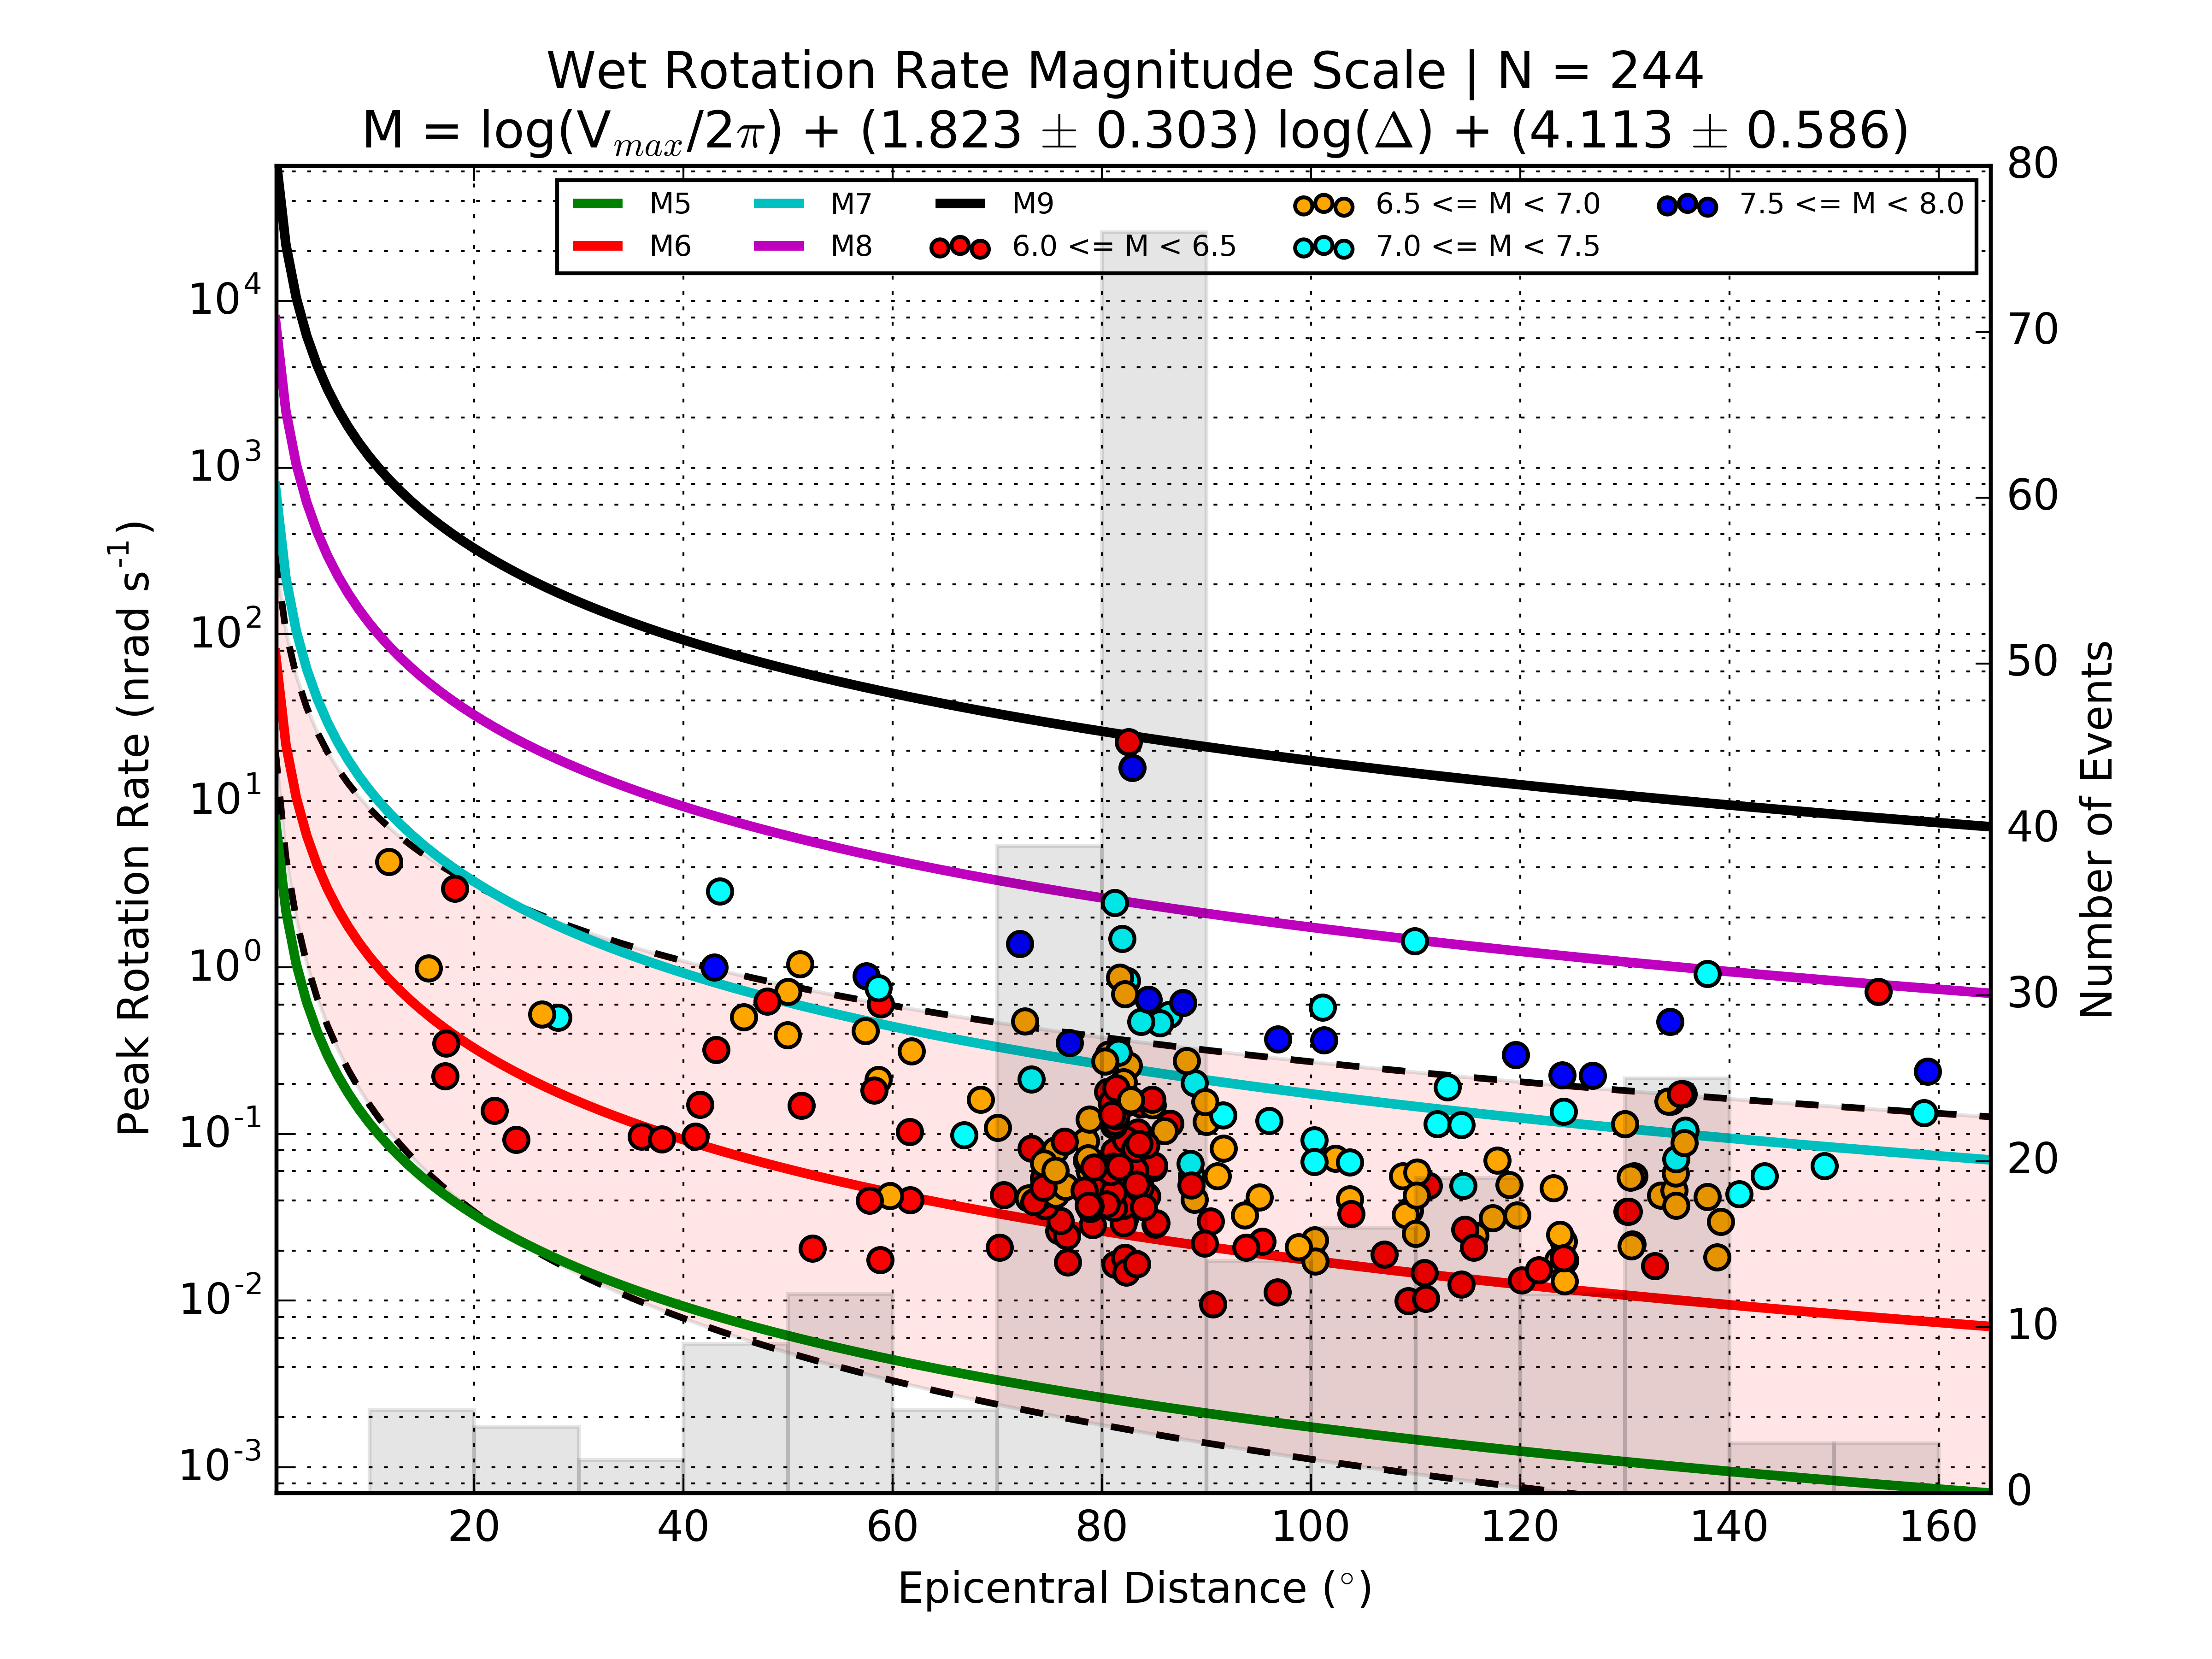
\includegraphics[width=.8\textwidth]{rr_obs}}
\caption{Rotation rate magnitude scale for observations. Event magnitudes separated by bins of 0.5 and denoted by color. Magnitude equation plotted by integer values as solid color lines. 95\% confidence interval for M6 shown by the shaded red area, bordered by black dashed lines. The number of events for each epicentral distance bin shown by gray bars in the background.}
\label{fig:rr_obs}
\end{figure*}


Table \ref{tab:scales} shows that the value of B covers a large range of values, ranging from 1.084 to 1.823 for vertical velocity M$^{WET}_{Z}$ and rotation rate M$^{RLAS}_{RR}$, respectively. Rotation M$^{RLAS}_{RT}$ falls closest to the standard IASPEI value of B, 1.66. Velocity values match quite consistently between Wettzell and F\"urstenfeldbruck, with FFB showing slightly higher amplitudes, as seen in the value of C, which controls the order of magnitude of each magnitude scale. A visual comparison of velocity scales can be seen in Figure \ref{fig:scale_comp}. 

\begin{figure}
\centerline{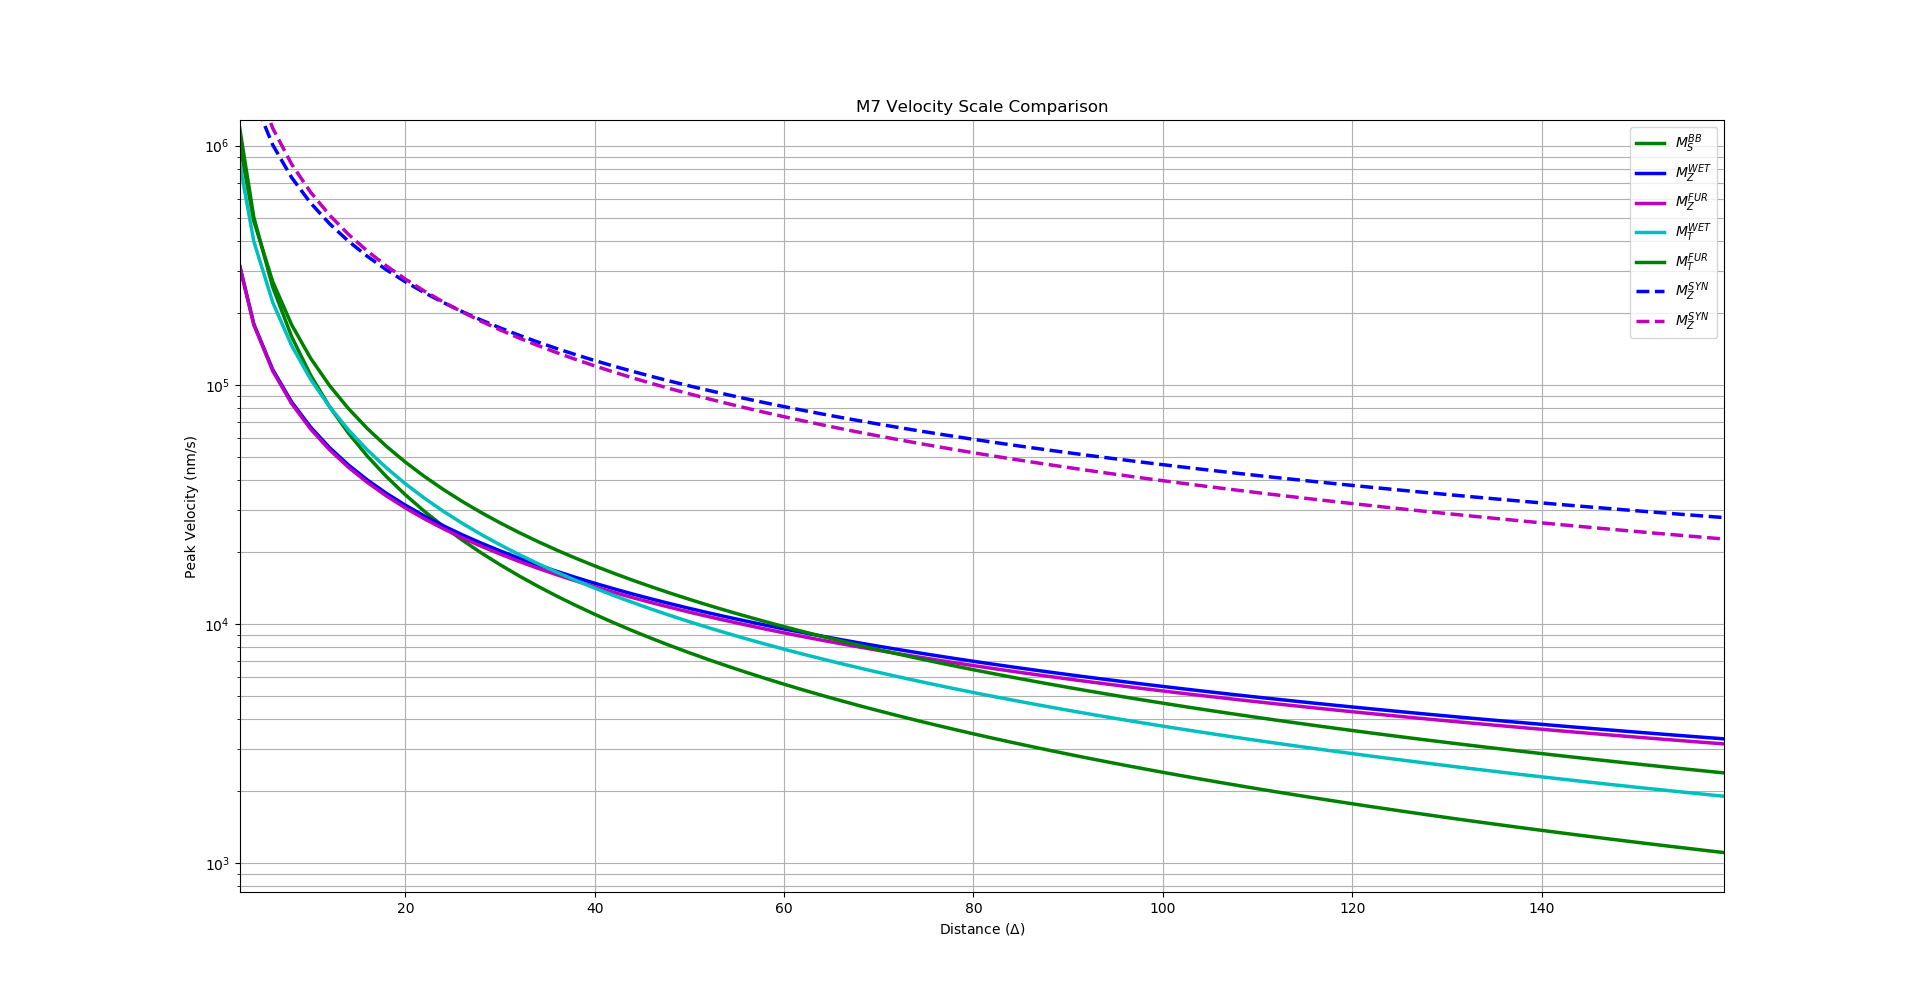
\includegraphics[width=.5\textwidth]{scale_compare}}
\caption{A comparison of velocity based scales for stations WET and FUR with the IASPEI scale used as reference. Peak amplitudes given in units of nanometers/s}
\label{fig:scale_comp}
\end{figure}

% in discussion?
It is to be expected that rotation rate would show a larger value for B as compared to rotation, as we are comparing rotation with its time derivative; rotation rate, containing higher frequency components compared to rotation, should exhibit quicker decay with distance as the earth filters out the high frequency energy. 

In these scales, there exists a drastic differences between values of B for velocity based scales. As the surface wave magnitude equation is defined for vertical component observations, the vertical velocity scale presents an identical setup as the broadband surface wave magnitude equation, however it gives here with the largest discrepancy, for both stations WET and FUR.  Transverse velocity, which should sample Love waves, same as rotations (see \ref{proxy}), shows a larger value for B as compared to vertical velocity, however it also exhibits lower than expected decay compared to the IASPEI scale. 

Confidence intervals, which can be viewed as a quantification of misfit between the fitted magnitude equation and the observations, shows the uncertainty of the observations due to the limitation of spatial coverage; in Figure \ref{fig:rr_obs}, the red shaded area shows the confidence interval of the magnitude 6 decay line. % add some explanation on confidence intervals
It should be noted that the magnitude scale is heavily controlled by the end points, i.e. very short and long distances. Due to a lack of events at very close epicentral distances, it is difficult to constrain the decay, and the few events that are at distances less than 20$^\circ$ have a strong influence on the derived value of B. It can also be seen that more than one third of the events used in this study fall around 80$^\circ$ epicentral distance, due to geographic constraints. Many of these events occur around Japan, and provide a good constraint of amplitudes at this distance.


%Discussion: comparing regional view vs an averaging
\subsection{Observed and synthetic waveforms}
For each of the 10 chosen events, synthetic seismograms were generated for all synthetic stations, as well as a 3$^\circ$ circle surrounding the event location, for very close observations. These results are left out of this study, however, as many of these synthetic stations would have been in the ocean, which presented a non-realistic scenario with which to compare our observations. Waveforms for station WET were compared for all components of translation and rotation to determine the accuracy of the simulation and 3D model. In most cases, P-wave arrivals matched exactly. Phases and amplitudes in the surface wave train, however, were not in agreement. Even for narrow pass filters, as in Figure \ref{fig:both}, observation and synthetic seismograms did not exhibit high correlations. Considerations should be made towards using point sources with no source time functions, % in discussion? 
and the rather broad range of frequencies included in the observations. Local site and source effects also may not have been taken into captured by the synthetic model used. Unfortunately due to limited computational resources, the synthetic traces only extend one hour, and do not capture the full extent of the waveform represented in the observations. Comparison of the waveforms, however, suggest that all of the surface wave energy has been captured in the one hour of simulation time. % perhaps compare waveforms for a smaller frequency band - t=20s?

\begin{figure}
\centerline{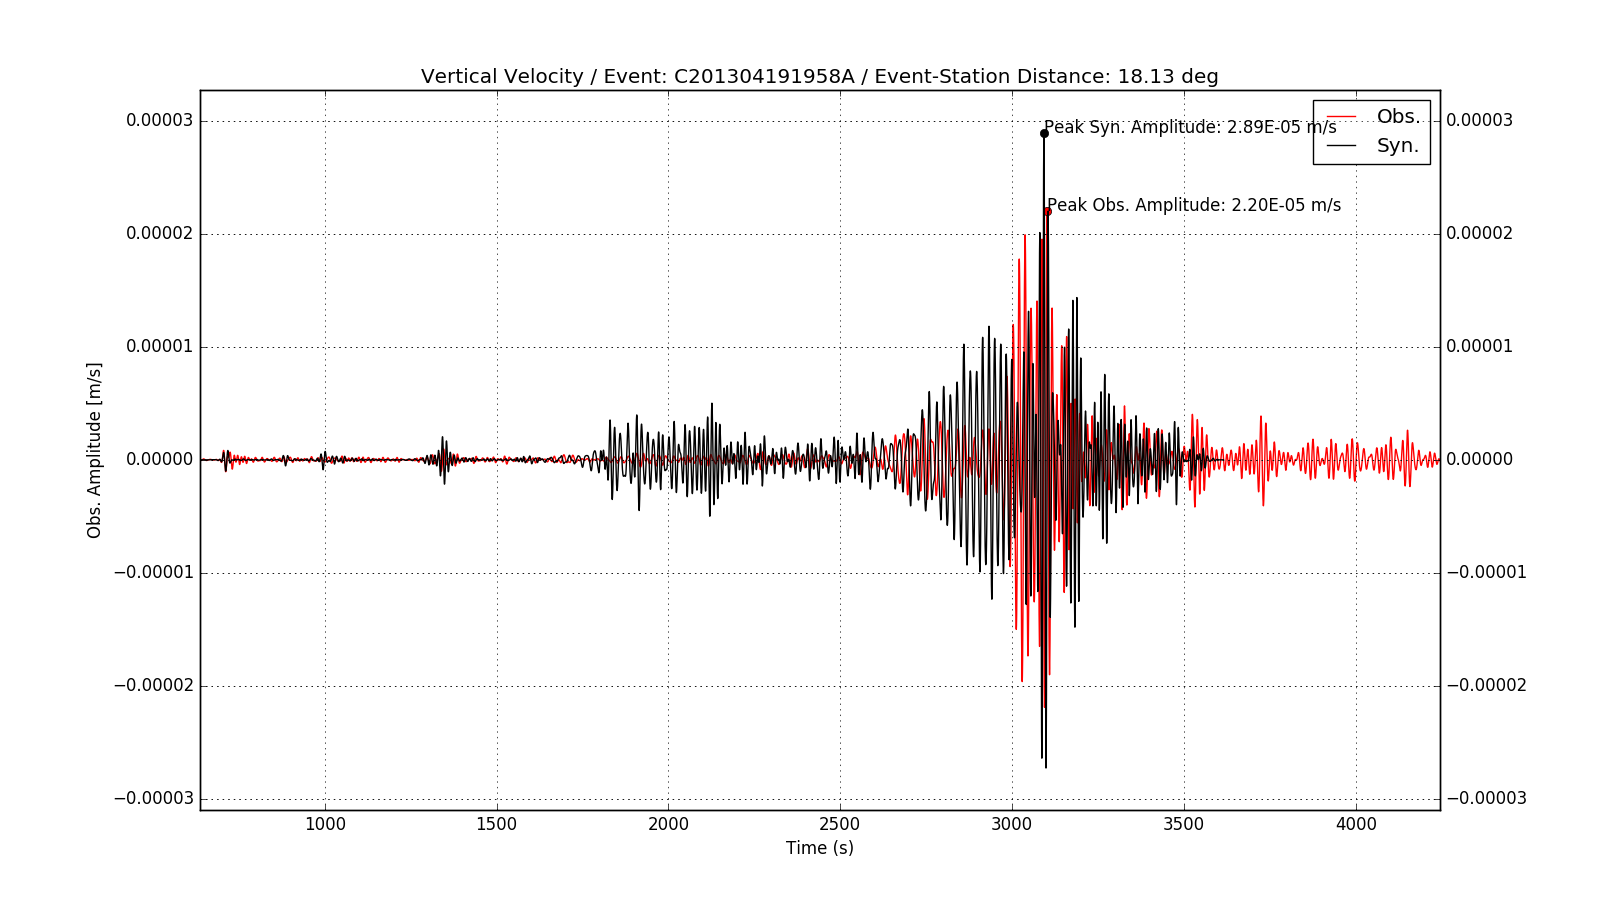
\includegraphics[width=0.5\textwidth]{both_waveformsC201304191958A}}
\caption{A comparison of synthetic and observed waveforms for an M6.1 event, East of Kuril Islands. Waveforms filtered at dominant period 20s.}
\label{fig:both}
\end{figure}

\subsection{Synthetic magnitude scales}
The derived magnitude scales for synthetic results differ drastically from the observed results. The synthetic results  do not reflect the same discrepancies that are present in the values given in Table \ref{tab:scales}.

Looking at Figure [SYN MAG SCALE FIG], the distribution of points on the magnitude scales is much more uniform. This can be attributed to the increased number of recordings for a single event due to the large number of synthetic stations. With so many station receiver pairs over a range of epicentral distances, it is possible for the receiver to track the earthquake. This was unfortunately not possible in the observations, and gives rise to some discrepancy in the appearance of the different magnitude scales. 

The synthetic magnitude scales all exhibit very similar values for the decay constant B. The large variation in decay as seen in the observations is not at all captured here. The largest discrepancy between two scales is X!. Even between rotation and rotation rate, as well as the values of velocity.

\begin{figure*}
\centerline{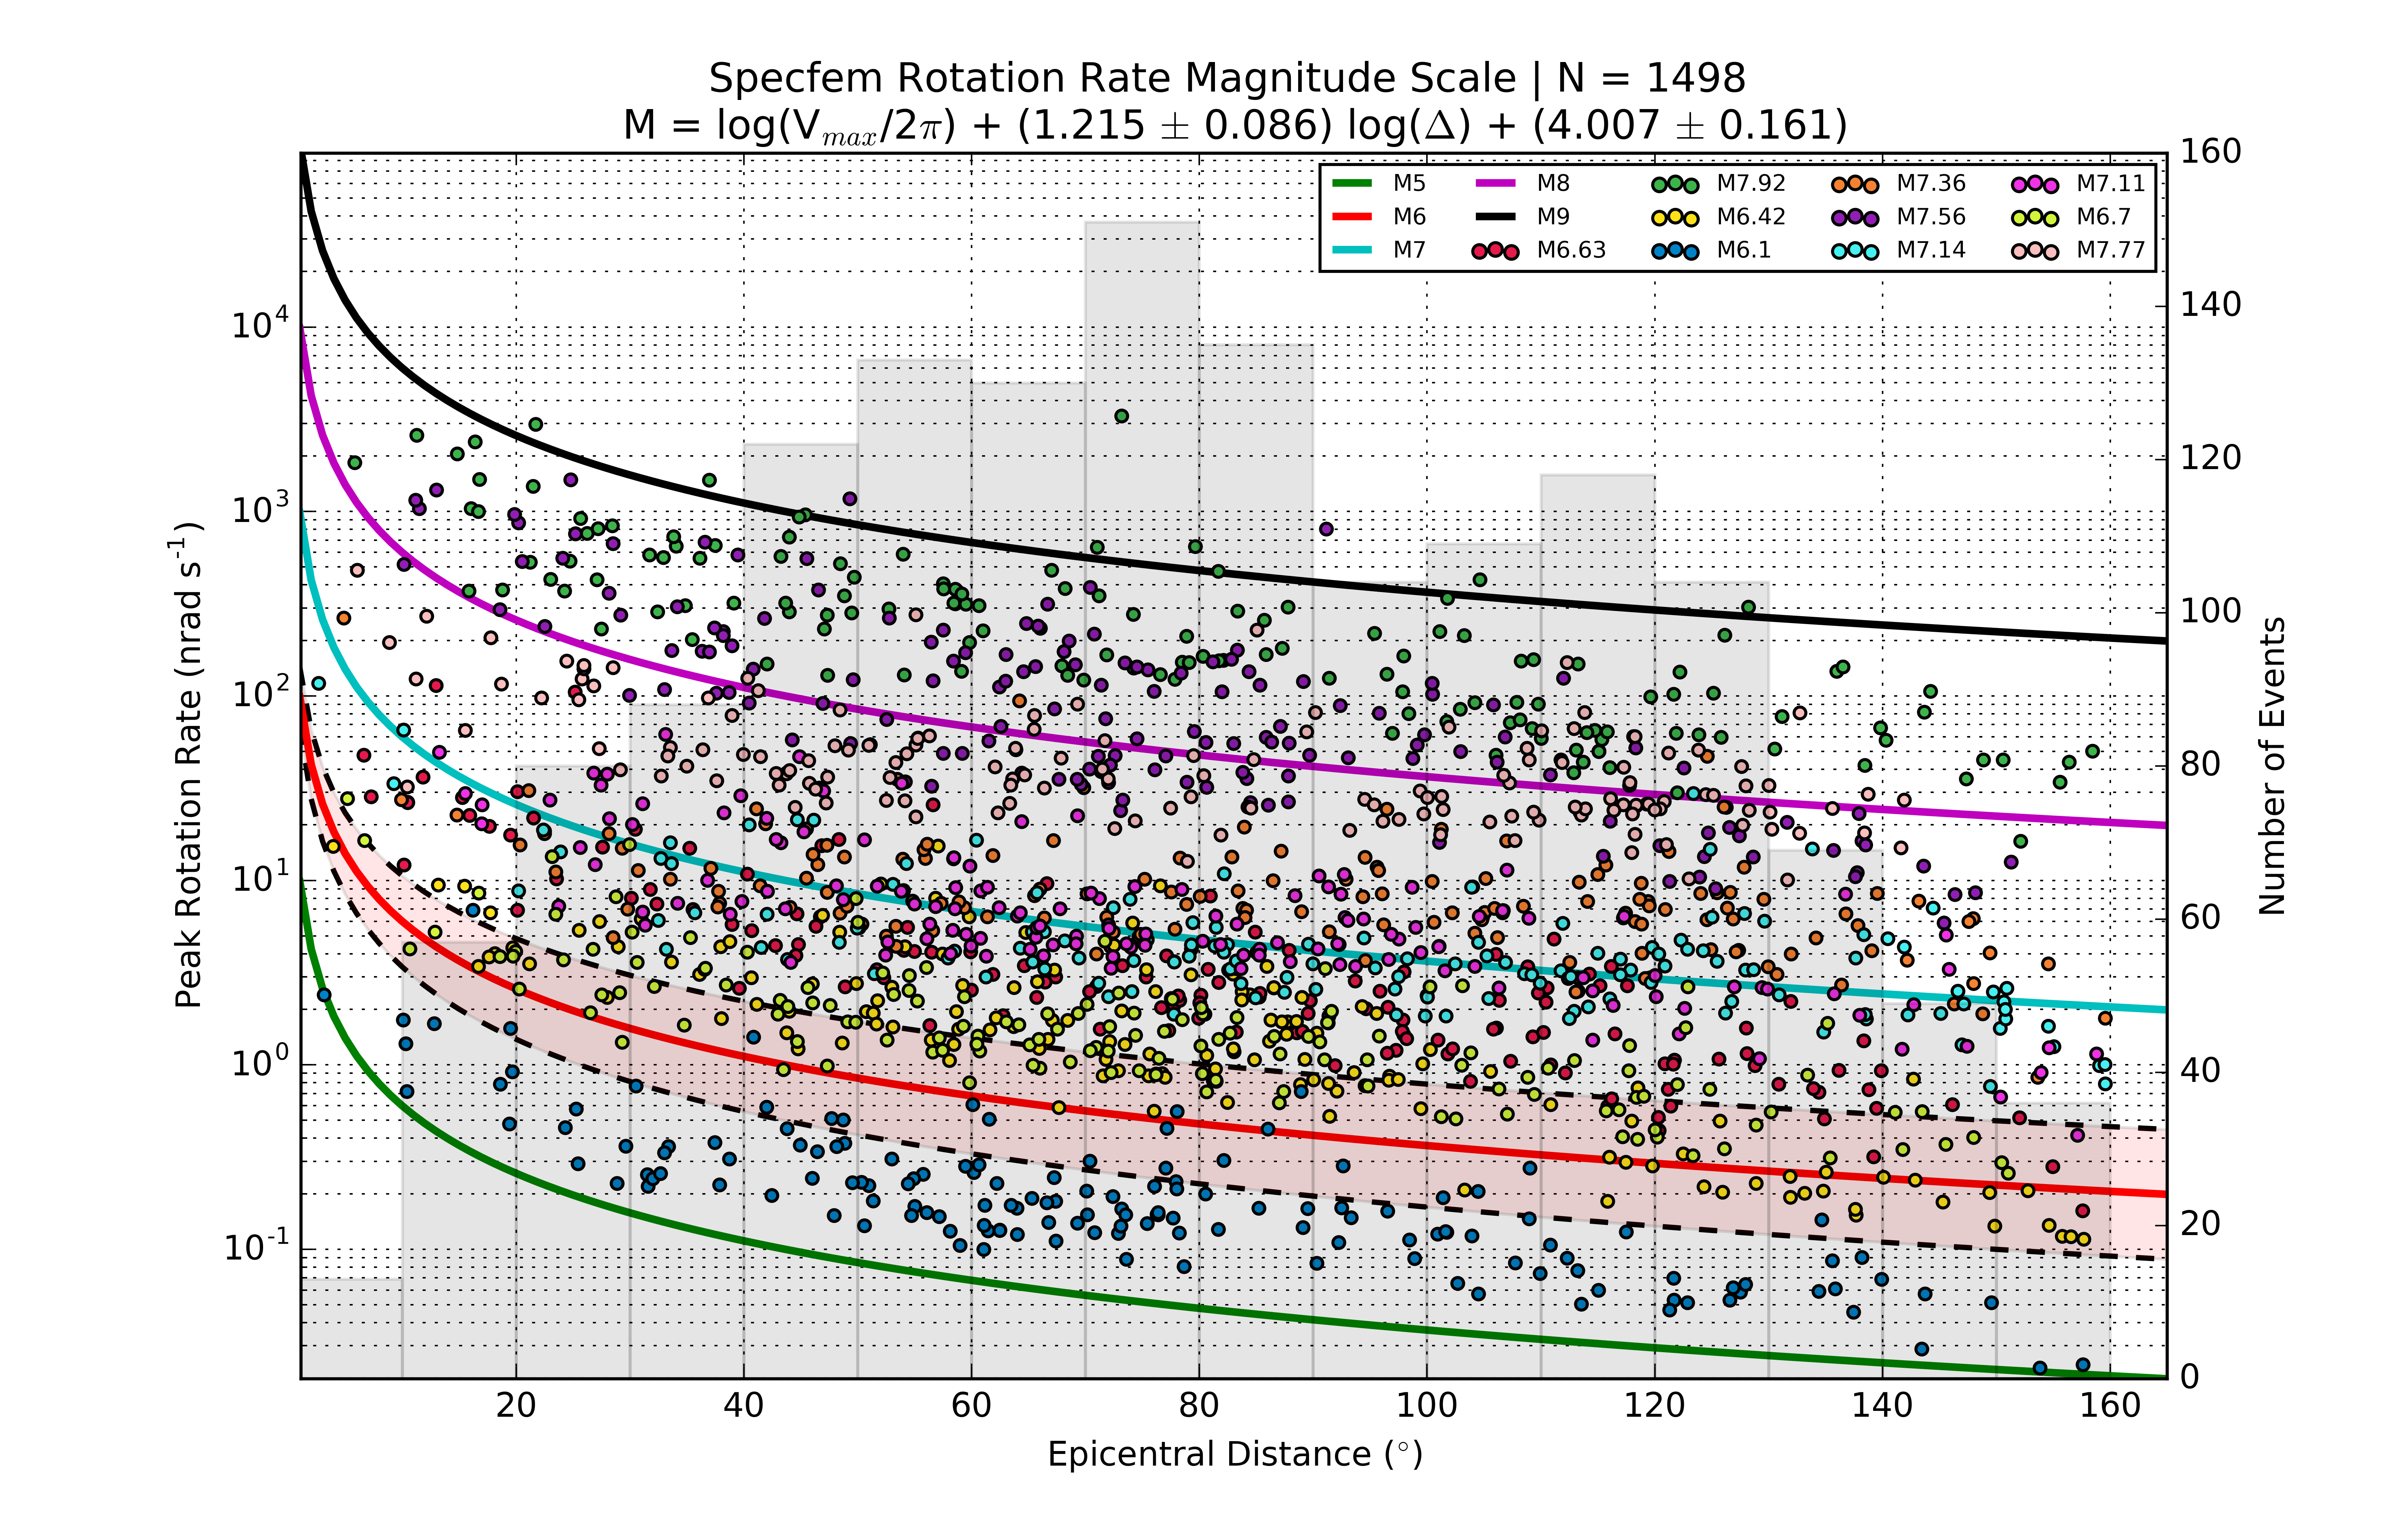
\includegraphics[width=0.8\textwidth]{rr_syn}}
\caption{Rotation rate magnitude scale for synthetics. All objects similarly represented as in Figure \ref{fig:rr_obs}. Colors of points here represent individual events simulated (for event information, see Table \ref{tab:syn_events}).}
\label{fig:syn_scale}
\end{figure*}

\begin{table*}
\begin{minipage}{115mm}
	\begin{center}
		\begin{tabular}{ |l|c|c|c|c| } 
		        \bf{Scale} & \bf{Label} & \bf{B} & \bf{C}  & \bf{Wave}\\ \hline
	IASPEI & $M_{S}^{BB}$ & 1.66 & 0.3  & Rayleigh \\ \hline
        Rotation  & $M^{RLAS}_{RT}$ & 1.557 $\pm$ 0.295 & 4.186 $\pm$ 0.569  & Love \\ \hline
	Rotation Rate & $M^{RLAS}_{RR}$ & 1.823 $\pm$ 0.303 & 4.113 $\pm$ 0.586  & Love\\ \hline 
        Transverse Velocity (Wettzell) & $M^{WET}_T$ & 1.45 $\pm$ 0.27 & 0.527 $\pm$ 0.521 & Love \\ \hline
        Transverse Velocity (FFB) & $M^{FUR}_T$ & 1.442 $\pm$ 0.27 & 0.447 $\pm$ 0.523 & Love \\ \hline
        Vertical Velocity (Wettzell) & $M^{WET}_Z$ & 1.084 $\pm$ 0.264 & 1.093 $\pm$ 0.511  & Rayleigh \\ \hline
        Vertical Velocity (FFB) & $M^{FUR}_Z$ & 1.095 $\pm$ 0.259 & 1.09 $\pm$ 0.502  & Rayleigh \\ \hline
		\end{tabular}
		
    		\caption{Magnitude scales and derived constants with 95\% confidence intervals for observations at instruments RLAS, WET (Wettzell, Germany) and FUR (F\"urstenfeldbruck, Germany), for equations of the form $M = log_{10}(V/2\pi) + B\cdot log_{10}(\Delta) + C$. The final column gives consideration to the wave type that each instrument component should provide a proxy for.}
		\label{tab:scales}
	\end{center}
	\end{minipage}
\end{table*}

\begin{table*}
\begin{minipage}{115mm}
	\begin{center}
		\begin{tabular}{ |l|c|c|c|c| } 
		        \bf{Scale} & \bf{Label} & \bf{B} & \bf{C}  & \bf{Wave}\\ \hline
        Synthetic Rotation  & $M^{SYN}_{RT}$ & 1.204 $\pm$ 0.086 & 3.841 $\pm$ 0.159  & Love \\ \hline
	Synthetic Rotation Rate & $M^{SYN}_{RR}$ & 1.215 $\pm$ 0.086 & 4.007 $\pm$ 0.161  & Love\\ \hline 
        Synthetic Transverse Velocity & $M^{SYN}_T$ & 1.094 $\pm$ 0.081 & 0.146 $\pm$ 0.16 & Love \\ \hline
        Synthetic Vertical Velocity  & $M^{SYN}_Z$ & 1.206 $\pm$ 0.08 & -0.011 $\pm$ 0.149  & Rayleigh \\ \hline
		\end{tabular}
		
    		\caption{Synthetic magnitude scales and derived constants with 95\% confidence intervals, for equations of the form $M = log_{10}(V/2\pi) + B\cdot log_{10}(\Delta) + C$. The final column gives consideration to the wave type that each instrument component should provide a proxy for.}
		\label{tab:syn_scales}
	\end{center}
	\end{minipage}
\end{table*}



\subsection{Expected rotation amplitudes}
One useful aspect of magnitude scales is to provide an expected amplitude value for a given magnitude event at certain distance. This is quite helpful in areas such as seismic hazard, where one can estimate the order of magnitude of ground motion at a location some distance away from an event, given a certain event size, though this is also dependent on site effects, travel paths, and amplitude modulation due to attenuation, focusing etc. This has largely been replaced by the concept of ground motion prediction equations, however in the emerging field of rotational seismology, it provides a useful insight.% something about GMPA

One concern in rotational seismology arises from whether or not newly developed field deployable rotation sensors will have the sensitivity necessary to capture the rotational motion amplitudes excited by regional or distant seismic events. With the rotational magnitude scale we derived here, we are able to create a list of expected rotational amplitudes for tele-seismic events. At the time of writing, the field deployable rotation sensor BlueSeis from the company iXBlue, has a noise floor of about (???) [Cite ???], which measures gradient information (rotation rate). Referring to the values given in Table \ref{tab:scales}, the maximum distance the sensor can be to detect a M$_w$ event would be X$^\circ$. Other considerations must be taken into account before these values can be used for field deployment decisions, however it provides a jumping off point for a new area of field research.


\section{Discussions and conclusions}
Long term continuous recordings of collocated rotation and translation now provides an extensive catalog of seismic events usable in comparisons of direct translation and spatial gradient measurements. Comparisons of phase information have been, and continue to be, explored in the context of seismology, but the measure of amplitudes has largely been ignored. Understandably, amplitude information is heavily dependent on a number of factors, including local site effects and even instrument characteristics, and does not provide as stable a measurement as phase information. However, by sampling a catalog of large, high quality seismic events with good spatial and temporal variability, as well as addressing the amplitude information via a log scale, which minimizes the impact of variations to order of magnitude differences, we hope to suppress the inherent instability of amplitude observations in order to make some quantitative statements on surface wave behaviors.

The results of this work, presented in Section \ref{sec:results}, provide a very interesting and unexpected picture, which we hope to address in this section.

 The results at face value show that observed rotations for the event catalog used decay faster than observed translations for the same events, and that rotation rate decays faster than the rotation, though this is to be excepted as we are simply looking at time derivative information. What is most interesting is how the rotation and rotation rate decays match much closer to the globally averaged surface wave magnitude as compared to the translation measurements which it is based off. Understandably a global average should be taken to give a more reasonable value for the decay. It should be pointed out, however, that even without global averaging, it is exciting to see the characteristics of this new observable, and by taking comparisons of direct measurements, we are gaining more understanding of the behaviors of this observable.

In this setup, multiple stations were used to record synthetic waveforms from single events, and as a result it is possible to see the amplitude decay of a single event over distance. 

%does this belong here?
Since we were not capable of this in the observable results, there is a stark difference in how the magnitude scales look and are derived. One major contrast between synthetics and observations is the differences in amplitudes of both rotational and translational motions. Given the magnitude equations in Tables \ref{tab:scales} and \ref{tab:syn_scales}, for an example event magnitude 7 at a distance of 100$^\circ$, we retrieve an expected rotation rate value of X for observations, but Y for synthetics. In the same vein, velocities show X and Y for observations and synthetics respectively.

Although amplitude differences were to be expected, these contrasts are quite strong. Possible explanations include the frequencies of interest or perhaps structural or site effects that are not modeled or captured by the synthetic mesh. %elaborate further


to add: 
-structure differences between ffb and wettzell
-high frequency attenutation of rotation rate compared to rotation
-herak and herak newly proposed magnitude scale
-averaging of earth structure not done here
-considerations towards using the correct backazimuth
-confidence interval

\label{lastpage}


\end{document}


%\begin{figure}[h]
%\centerline{\includegraphics[width=0.8\textwidth]{XYZ}}
%\caption{XYZ}
%\end{figure}
